% FHE 31 May 2025 copied from rt/rt-notes/intro-and-logistic-note.tex
\documentclass[11pt]{article}
%% \usepackage{hyperref}
\usepackage{graphicx}
\usepackage{svg}
\usepackage[nohead,marginratio={1:1,1:1},vscale=0.73]{geometry}
%% \usepackage[nohead,nofoot,marginratio={1:1,1:1},vscale=0.7]{geometry}

% FHE 14 Sep 2024
% copied from /home/frederik/rt-patent/preprint-files/rt-preprint.tex
\usepackage{amsfonts}
\usepackage{amsmath}
\newcommand{\T}{\top}
\newcommand{\bb}[1]{\mathbb{ #1 }}
\newcommand{\R}{\bb{R}}
\newcommand{\norm}[1]{\lVert #1 \rVert}
\newcommand{\abs}[1]{\left| #1 \right|}
\renewcommand{\(}{\left(}
\renewcommand{\)}{\right)}
\newcommand{\argmax}{\mathop{\mathrm{argmax}}}
\newcommand{\argmin}{\mathop{\mathrm{argmin}}}
\renewcommand{\L}{\mathcal{L}}
\newcommand{\partby}[2]{{\partial #1\over \partial #2}}
\newcommand{\partbyby}[3]{{\partial^2 #1\over \partial #2 \partial #3}}
\newcommand{\partbyt}[2]{{\partial^2 #1\over {\partial #2}^2}}
\newcommand{\ud}{\mathrm{d}}
\newcommand{\dby}[2]{\frac{\ud #1}{\ud #2}}
\newcommand{\dbyt}[2]{\frac{\ud^2 #1}{{\ud #2}^2}}
\newcommand{\eps}{\varepsilon}
\newcommand{\ditto}{\texttt{"}}
\newcommand{\I}{\mathcal{I}}
\newcommand{\Iup}{\I_{\textrm{up,params}}}
\newcommand{\Iul}{\I_{\textrm{up,loss}}}
\newcommand{\Iur}{\I_{\textrm{up,reg}}}
\newcommand{\zt}{z_{\textrm{test}}}
\newcommand{\zu}{z}
%% \newcommand{\zu}{z_{\textrm{up}}}
% what symbol are we using for gradient of loss?
\newcommand{\gl}{\sigma}
%\newcommand{\gl}{\lambda}  %% better notation?
% expectation
\newcommand{\E}{\bb{E}}
\renewcommand{\l}{l} % LiSSA shorthand
\newcommand{\h}{h} % LiSSA shorthand
\renewcommand{\Gamma}{\textrm{Gamma}}
\newcommand{\where}{\:\big|\:}

\newcommand{\dottheta}{\dot{\theta}}

\newcommand{\betapr}{\beta^{\mathrm{PR}}}

\author{Frederik Eaton}
\date{31 May, 2025}
\title{Notes on NLCG design and implementation}

\begin{document}
\maketitle
%% \raggedright
%% \raggedbottom

The optimization procedure is the heart of any machine learning
application and deserves special consideration. The NLCG (Nonlinear
Conjugate Gradient) optimization algorithm is efficient in both time
and memory and seems difficult to improve upon, although at the same
time hard to understand. To make the code more understandable and
maintainable it seemed wise to include a short summary and
justification of the NLCG algorithm. Our primary reference is
Shewchuk, 1994, ``An Introduction to the Conjugate Gradient Method
\ldots''. Any page numbers in this document are referring to that
paper.

\tableofcontents

\section{The problem setup}

In the functional form of CG and NLCG we are minimizing (p.~2) the
quadratic form
\begin{align}
f(x) = {1\over 2} x^\T A x - b^\T x + c
\end{align}
The minus sign is from Shewchuk and relates to the matrix form of the
minimization problem,
\begin{align}
Ax=b
\end{align}
The CG method calculates $x=A^{-1} b$. The NLCG method applies to a
more general objective function $f$, which can be arbitrary if smooth,
and minimizes it. In this case $A$ will be the Hessian
$\partbyt{f}{x}(x)$ and $b$ the negative gradient at 0: $b=-f'(0)$.

It seems most sensible to motivate the NLCG optimization procedure
using some simple derivations from calculus, although the language in
Shewchuk uses more linear algebra; for example he calls the negative
gradient is called the ``residual'' $r$.

\section{Derivations}

\newcounter{deriv}
\newcommand{\deriv}[1]{
  \refstepcounter{deriv}
    \vspace{1em}
    \noindent\textbf{Derivation \thederiv: #1} \\
}

%\newcommand{\deriv}[1]{\item{\bf \value{enum} #1}\nopagebreak}

%\begin{enumerate}
\deriv{Whether stepping in a given direction will take us downhill}
\begin{align}
\left.\dby{}{\alpha}f(x+\alpha d) \right|_{\alpha=0} = f'(x)^\T d
\end{align}
If the inner product of $d$ with the gradient is negative, then a
small motion in the direction of $d$ will take us downhill. \label{downhill}

\deriv{The optimal step distance to take in any given direction}
From derivation 1, after taking an optimal step in direction $d$, the inner product of $d$ with the new gradient will be 0:

\begin{align}
  0 &= f'(x+\alpha d)^\T d \\
  &= (A(x+\alpha d)-b)^\T d \\
  &= (f'(x)+\alpha A d)^\T d \\
\implies  \alpha &= -{f'(x)^\T d \over d^\T A d}
\end{align}

Here $Ad$ can be calculated as an HVP at little cost.\footnote{It
seems that Shewchuk does not know about how to calculate the HVP
without the Hessian, see his arguments on p.~46 for example; in fact
his entire 1994 article never mentions backpropagation either, which
had been well described by the mid-1980s.} This is equivalent to
Newton's method in 1 dimension. The denominator could be written
$\left. \dbyt{}{\alpha}f(x+\alpha d) \right|_{\alpha=0}$ just as the
numerator is $\left. \dby{}{\alpha}f(x+\alpha d) \right|_{\alpha=0}$.

% figures from p. 14 and p. 32
\begin{figure}[h]
\parbox{\textwidth}{
  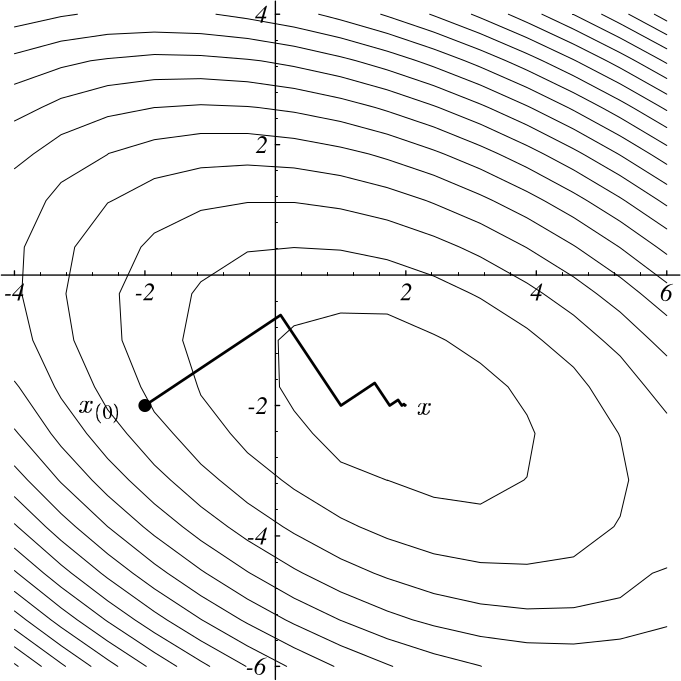
\includegraphics[width=0.45\textwidth]{images/shewchuk-p-8.png}
  \hfill
  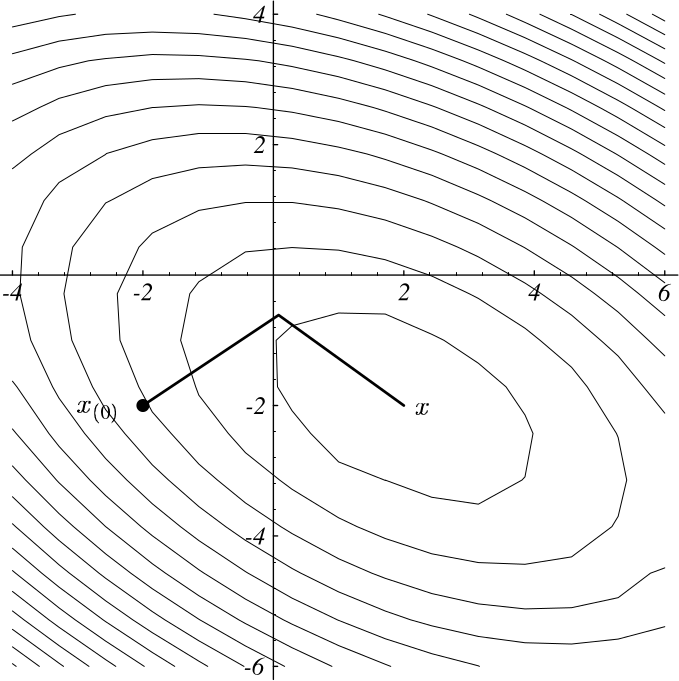
\includegraphics[width=0.45\textwidth]{images/shewchuk-p-32.png}
}
\caption{Steepest descent (left) versus Conjugate gradients (right).
  Copied from p.~8 and p.~32 of Shewchuk.}
\end{figure}

\deriv{How to avoid undoing our progress when we take the next step}
Consider $g(\alpha,\beta)=f(x+\alpha d + \beta e)$, and let
$\beta^*(\alpha)=\min_\beta g(\beta,\alpha)$. What we want is to
choose direction vectors $d$ and $e$ such that the optimal $\beta$
does not depend on our choice of $\alpha$:
$\dby{}{\alpha}\beta^*(\alpha) = 0$. By the implicit function theorem,
we have
\begin{align}
0 &= \dby{}{\alpha}\beta^* = -(\partbyt{g}{\beta})^{-1} (\partbyby{g}{\alpha}{\beta}) \\
&= -(e^\T A e)^{-1} (d^\T A e) \\
\implies d^\T A e &= 0
\end{align}
This is to say that vectors $d$ and $e$ are {\em conjugate} relative to $A$,
or we sometimes say $A$-perpendicular or $A$-orthogonal. Thus if we
choose successive direction vectors to be conjugate to all previous
ones (relative to $A$), then we can avoid backtracking. Note that the
order of steps does not matter when the directions are conjugate, as
each step length remains optimal independently of the others. In
particular the gradient condition in derivation 1 will hold for all
previous directions, implying that the new gradient will be
perpendicular to each of them.

\deriv{How to pick a new direction vector} At each step of our
optimization, we want as we have seen to choose a search direction
that is conjugate or $A$-perpendicular to all previous directions. The
natural quantity from which to derive the new direction is the
gradient $-r_n$, which is already perpendicular to all previous
directions $d_j : j\in [1,n-1]$. We can use HVPs with $A$ and
$d_{n-1}$ to project $r_n$ onto the subspace which is
$A$-perpendicular to $d_{n-1}$, and propose this as the next search
direction $d_n$:
\begin{align}
d_n &= r_n + \beta_n d_{n-1} \\
d_1 &= r_1
\end{align}
The HVPs appear when we solve\footnote{The expression on p.~32 of Shewchuk is
different, it is given as $\beta_n = {r_n^\T r_n \over r_{n-1}^\T
  r_{n-1}}$, which as we show later is equivalent to ours.} for
$\beta_n$:
\begin{align}
d_n A d_{n-1} & = 0  \\
\implies r_n A d_{n-1} + \beta_n d_{n-1} A d_{n-1} &= 0  \\
\implies \beta_n &= -{r_n A d_{n-1} \over d_{n-1} A d_{n-1}}
\end{align}

With this choice of $d_n$, we can show that conjugacy is obtained with
respect to all previous search directions as well. This is because the
new subspace $D_n$, spanned by the search directions up to $d_n$,
contains a copy of $A D_{n-1}$, implying that $r_{n+1}$, which is
perpendicular to $D_n$, will be A-perpendicular to $D_{n-1}$. More
precisely, for the step $x_{n+1} = x_n + \alpha_n d_n$, we can use the
following recurrence for the negative gradient:
\begin{align}
r_{n+1} &= r_n - \alpha A d_n \label{eq:radnrec} \\
\implies A d_n &= {1\over \alpha}(r_n - r_{n+1}) \label{eq:adnrndiff}
\end{align}
But if the next direction vector is always projected from $r$, then
$r_n = d_n - \beta_n d_{n-1}$ from above, so \ref{eq:adnrndiff} becomes
\begin{align}
A d_n = {1\over \alpha} (d_n -\beta_n d_{n-1}-(d_{n+1}-\beta_{n+1}d_n)) \label{eq:adn}
\end{align}
We have written $A d_n$ as a linear combination of $d_{n+1}$, $d_n$,
and $d_{n-1}$. Since, from the previous derivations, $r_n \perp d_j$
for $j\leq n-1$, equation \ref{eq:adn} implies that for $j\leq n-2$,
\begin{align}
r_n \perp D_{j+1} \implies r_n \perp A d_j
\iff r_n A d_j = 0
\end{align}
This says $r_n$ is A-perpendicular to $d_{n-2}$ and all earlier
directions. Assuming by induction that $d_{n-1}$ has this same
property, i.e.~$d_{n-1}A d_j=0$ for $j\leq n-2$, we find that when $d_n$ is formed
from a linear combination of $r_n$ and $d_{n-1}$ so as to be
$A$-orthogonal to $d_{n-1}$, it will also be A-orthogonal to all
previous $d$'s, $d_1$, \ldots $d_{n-2}$, as both $r_n$ and $d_{n-1}$
have this (linear) $A$-orthogonality property with the subspace
$D_{n-2}$.

%\end{enumerate}

\section{The algorithm and its variations}

From the foregoing observations we can write down the steps of the CG
or NLCG algorithm, given an input $f$ which is approximately
quadratic, and a starting point $x_1$.
\begin{align}
r_1 &= -f'(x_1) \\
d_1 &= r_1 \\
x_n &= x_{n-1}+\alpha_{n-1}d_{n-1} \\
r_n &= -f'(x_n) \\
d_n &= r_n + \beta_n d_{n-1}
\end{align}
where
\begin{align}
\alpha_n &= -{f'(x_n)^\T d_n \over d_n^\T A d_n}
\textrm{\quad from derivation 2} \\
\beta_n &= -{r_n A d_{n-1} \over d_{n-1}A d_{n-1}}
\textrm{\quad from derivation 4} \\
\end{align}
We can calculate all of these quantities efficiently if we keep track
of the HVP $A d_n$ at each step. However, it is possible to use the
orthogonality properties of $d_j$ and $r_j$ to rewrite some of the
HVPs, following Shewchuk, from \ref{eq:radnrec}:
\begin{align}
\beta_n &= -{r_n^\T A d_{n-1} \over d_{n-1}^\T A d_{n-1}} \\
 &= -{r_n^\T (r_{n-1}-r_n) \over d_{n-1}^\T (r_{n-1}-r_n)}
\end{align}
But $r_n^\T r_{n-1} = r_n^\T(d_{n-1}-\beta_{n-1}d_{n-2}) = 0$ and
$d_n^\T r_n = (r_n + \beta_n d_{n-1})^\T r_n = r_n^\T r_n$, so
\begin{align}
\beta_n = {r_n^\T r_n \over r_{n-1}^\T r_{n-1}} \label{eq:r-beta}
\end{align}
is equivalent and has no HVPs in it. The expression Shewchuk uses for
$\alpha_n$, however, includes an HVP in the denominator because the
new gradient $r_{n+1}$ is not available at this stage of the
computation. Only the numerator is rewritten:
\begin{align}
\alpha_n &= {r_n^\T d_n \over d_n^\T A d_n} \\
&= {r_n^\T r_n \over d_n^\T A d_n}
\end{align}
Shewchuk advocates recalculating the gradient at each step of the NLCG
algorithm on p.~42,
\begin{align}
r_n = -f'(x_n)
\end{align}
but for the CG algorithm he uses the recurrence
\ref{eq:radnrec}:
\begin{align*}
r_{n+1} &= r_n - \alpha_n A d_n
\end{align*}
With these modifications, we have the CG algorithm from p.~32 of
Shewchuk. The NLCG algorithm as he presents it is only different in
that (1) it computes $r_n$ anew at each step, as the negative
gradient, (2) it recommends using the Polak-Ribiere $\betapr$ and
restarts (\ref{eq:betapr}) rather than the simpler Fletcher-Reeves
$\beta$ (\ref{eq:r-beta}).

We are not sure which of these alterations to the ``naive''
formulation of CG is necessary or useful in the context of non-linear
optimization. For example the HVP $A d_n$ can be computed together
with the gradient $-r_n=f'(x_n)$, so it is not more efficient to use a
recurrence for $r_n$ unless we can isolate the dual part of a
computation (\verb|tape_get_dual|) and compute only the HVP; but this
seems only advantageous if $x$ is constant as it is in our dual-number
interpretation of CG.

The choice of step length $\alpha$ can be as above in the CG
algorithm, although Shewchuk advocates a more general line search to
reliably minimize $f(x+\alpha d)$ with respect to $\alpha$. This could
also involve additional Newton steps on $\alpha$, or the secant method
(p. 52 and 53). Reliably minimizing $\alpha$ helps guarantee that the
new gradient is orthogonal to the last search direction, so that the
assumptions of the algorithm continue to hold, but on the other hand
if we are adjusting $\alpha$ to step out of a concavity then the old
Hessian $A$ is unlikely to describe the curvature at the new $x$ in
the first place.\footnote{If we find ourselves in a concavity, then
we might as well step out of it in a totally random direction.
Although it is tempting to make use of the curvature, and for example
take a step which is the exact opposite of the step that would take us
to the local maximum.}

The projection coefficient $\beta_n$ is often calculated as
\begin{align}
\betapr_n &= {r_n^\T (r_n-r_{n-1}) \over r_{n-1}^\T r_{n-1}} \label{eq:betapr}
\end{align}
which is called the Polak-Ribiere formula. (Equation \ref{eq:r-beta}
is called the Fletcher-Reeves formula)

This choice of $\beta$ gives us ``restarts'' if we set
$\beta=\max\{\betapr,0\}$. The event of $\beta$ becoming nonpositive
generally happens when we have exhausted all the search directions,
but we are not sure why this is so.

Interestingly, if $A=I$ then we will never build up a basis of
conjugate directions; but we won't need to, as the gradient will
always point at the optimum.

\section{Thoughts on extending NLCG}

It is hard to think of a good multidimensional generalization of NLCG,
as we are already effectively doing a Newton step at each NLCG
restart. My March 18 2025 ``regularity tangent'' preprint on p.~34
speculates about such a generalization and outlines an algorithm based
on a linear embedding, but this algorithm concept introduces
additional overhead that seems unnecessary. NLCG is able to propose
direction vectors one at a time, while still effectively inverting the
Hessian, with a sequence of 1-dimensional Newton steps.

There must be a way to make NLCG work ``stochastically'', i.e.~ with
batches, but presumably these should stay the same until the next
restart. It could be trusted to make (close to) the smallest possible
adjustment to the parameters to give the model good performance on the
current batch. Then the NLCG restarts would be like a heartbeat, and the
current batch of data would be all the blood that fits into the
``heart'', and each restart would trigger a new batch to be called up.
However this would be a problem with regularized models as the
successive batches would fight with each other over the parameter
vector's expressiveness.

A simple solution would be to create a kind of memory using
$\abs{\theta-\theta_0}$ regularization where $\theta_0$ is from the
end of the previous batch. The regularizer can be adjusted using the
previous batch as a test set for example, and making slight
adjustments up or down according to the $\dby{}{s}$ of the test error.
Or we can curate a test set as we go using the RT. But we should have
a traditional regularizer as well, and control the ratio of the
regularization coefficients. And note that this can be done in a
hierarchy; for example a separate parameter vector for the current
hour, minute, and second.

NLCG should refuse to increase the objective. It is not clear what to
do when this happens. If the gradient indicates the objective should
decrease, then we can reduce the step size until we find a decrease
from the current value. If however the Newton step on $\alpha$ is
pointing us uphill, then this indicates we're in a local concavity,
and it would make sense to try walking the same distance in the other
direction before we even update $x$ and calculate the new objective.
In either case we may want to try larger and larger steps if the last
step is successful, and smaller ones (or break out of the loop) if it
isn't. Once a minimum is bracketed, the secant method or Newton's
method can be used to pinpoint it, but it is not clear that this extra
effort would be useful, as a restart would seem to be called for at the
point where we find the objective increasing.

\section{Automatic differentiation of optimization}

In the context of non-linear optimization, the (linear) conjugate
gradients method can best be thought of as an algorithm for inverting
the dual of the objective gradient with respect to the dual of the
optimal independent variable ($x^*$). An input consists of an optimum
$x^*$, an objective function, and a target dual gradient $-b$.

\newcommand{\xdot}{\dot{x}}

The algorithm finds an $\xdot$ such that $A\xdot = b$, which is to say
that $\dby{}{\eps} \partby{}{x} f(x^* + \eps \xdot) =
\dby{}{\eps}(A(x^*+\eps \xdot)-b) = A\xdot$, which is the
Hessian-vector product at $x^*$ of $f$ with $\xdot$, should equal the
target value $b$. (In this setting, $b$ is an input to the algorithm
rather than part of the objective $f$) Each
iteration updates $\xdot$ and computes a new HVP, always at the same
$x=x^*$. It is necessary to compute a HVP with the direction
vector $d$ in order to determine the step length $\alpha$ and the
quotient coefficient $\beta$ for the conjugate projection, although
the latter can be approximated as a difference of successive gradients
as in equation \ref{eq:adnrndiff} to get the Fletcher-Reeves formula
\ref{eq:r-beta} with no HVP.

The CG algorithm can be used to apply the implicit function theorem to
an optimization problem. Once an optimum $x^*$ is found via NLCG, we
can calculate total derivatives by using plain CG to approximate the
inverse-HVP of Cauchy's implicit function theorem:
\begin{align}
  x^*(t) &=  \argmin_x f(x,t) \\
\dby{}{t}x^*(t) &= -\left(\stackrel{A}{\overbrace{\partbyt{}{x}f(x^*,t)}}\right)^{-1} \stackrel{b}{\overbrace{\partbyby{}{x}{t}f(x^*,t)}} \label{eq:ift}
\end{align}
In this case $b$, which along with $f$ is the input to the CG
algorithm, is calculated as the derivative of the gradient
$\partby{f}{x}$ with respect to the hyperparameter $t$. At first
glance, if there is more than one hyperparameter or if $t$ has more
than one dimension, then it seems that multiple inverse-HVPs will be
required, implying multiple runs of CG. However, when backpropagating
adjoints through an optimization run, we can make use of the symmetry
of $A$ to make do with only a single inverse-HVP, involving the
adjoint of $x^*$. Taking the inner product of \ref{eq:ift} with the
incoming adjoint $\dby{y}{x^*}$:
\begin{align}
  \dby{y}{t} = \dby{y}{x^*}^\T \dby{}{t}x^* &= -\dby{y}{x^*}^\T \left(\partbyt{f}{x} \right)^{-1} \partbyby{f}{x}{t} \\
  &= -\dby{}{t}\left(\underbrace{\left( A^{-1} \dby{y}{x^*} \right)^\T}_{{\textrm{\tiny treat as} \atop \textrm{\tiny constant}}}\partby{f}{x}\right)
\end{align}

So the derivatives of all hyperparameters can be calculated by
backpropagating adjoints from the ``pseudo-objective'' above, which is
constructed from the function gradient and the inverse HVP of the
incoming adjoint $\dby{y}{x^*}$. The recipe becomes: First use CG to
calculate the inverse HVP $A^{-1} \dby{y}{x^*}$; then, treating this
as a constant, take its inner product with the function gradient at
$x^*$. Take the result as an objective and backpropagate adjoints from
it to all the hyperparameters $t$. We are not sure, but this must be
related to the methods proposed in Lorraine, Vicol, and Duvenaud,
2020, ``Optimizing Millions of Hyperparameters by Implicit
Differentiation''. This is the key to an efficient
``\verb|back_opt_nlcg|'' corresponding to backpropagation through NLCG
optimization. For the corresponding forward-derivative
``\verb|dual_opt_nlcg|'' function we can use the non-zero dual
components to calculate $-b=\partbyby{f}{x}{t}$ (where $t$ is the dual
variable) and pass this through $A^{-1}$ more straightforwardly in a
single run of CG.

\end{document}
